
\documentclass{beamer}
\usecolortheme{dove}
\setbeamertemplate{navigation symbols}{}
\usepackage{amsmath,amssymb,amsfonts,amsthm, multicol, subfigure, color}
\usepackage{bm}
\usepackage{graphicx}
\usepackage{tabularx}
\usepackage{booktabs}
\usepackage{hyperref}
\usepackage{pdfpages}
\usepackage{xcolor}
\definecolor{seagreen}{RGB}{46, 139, 87}
\def\independenT#1#2{\mathrel{\rlap{$#1#2$}\mkern2mu{#1#2}}}
\newcommand\indep{\protect\mathpalette{\protect\independenT}{\perp}}
\def\log{\text{log}}
\newcommand\logit{\text{logit}}
\newcommand\iid{\stackrel{\text{iid}}{\sim}}
\newcommand\E{\text{E}}
\newcommand\V{\text{V}}
\renewcommand\P{\text{P}}
\newcommand{\Cov}{\text{Cov}}
\newcommand{\Cor}{\text{Cor}}
\newcommand\doop{\texttt{do}}
\usepackage{stackrel}
\usepackage{tikz}
\usetikzlibrary{arrows,shapes.arrows,positioning,shapes,patterns,calc}
\newcommand\slideref[1]{\vskip .1cm \tiny \textcolor{gray}{{#1}}}
\newcommand\red[1]{\color{red}#1}
\newcommand\blue[1]{\color{blue}#1}
\newcommand\gray[1]{\color{gray}#1}
\newcommand\seagreen[1]{\color{seagreen}#1}
\newcommand\purple[1]{\color{purple}#1}
\newcommand\orange[1]{\color{orange}#1}
\newcommand\black[1]{\color{black}#1}
\newcommand\white[1]{\color{white}#1}
\newcommand\teal[1]{\color{teal}#1}
\newcommand\magenta[1]{\color{magenta}#1}
\newcommand\Fuchsia[1]{\color{Fuchsia}#1}
\newcommand\BlueGreen[1]{\color{BlueGreen}#1}
\newcommand\bblue[1]{\textcolor{blue}{\textbf{#1}}}
\newcommand\bred[1]{\textcolor{red}{\textbf{#1}}}
\newcommand\bgray[1]{\textcolor{gray}{\textbf{#1}}}
\newcommand\bgreen[1]{\textcolor{seagreen}{\textbf{#1}}}
\newcommand\bref[2]{\href{#1}{\color{blue}{#2}}}
\colorlet{lightgray}{gray!40}
\pgfdeclarelayer{bg}    % declare background layer for tikz
\pgfsetlayers{bg,main} % order layers for tikz
\newcommand\mycite[1]{\begin{scriptsize}\textcolor{darkgray}{(#1)}\end{scriptsize}}
\newcommand{\tcframe}{\frame{
%\small{
\only<1|handout:0>{\tableofcontents}
\only<2|handout:1>{\tableofcontents[currentsubsection]}}
%}
}

\usepackage[round]{natbib}
\bibliographystyle{humannat-mod}
\setbeamertemplate{enumerate items}[default]
\usepackage{mathtools}

\newcommand{\goalsframe}{\begin{frame}{Learning goals for today}
At the end of class, you will be able to:
\begin{enumerate}
\item Gain efficiency with marginal structural models
\item Recognize how that gain comes through information sharing
\item Understand stabilized weights
\end{enumerate} \vskip .2in
\end{frame}}

\title{14. Marginal Structural Models}
\author{Ian Lundberg\\Cornell Info 6751: Causal Inference in Observational Settings\\Fall 2022}
\date{6 Oct 2022}

\begin{document}

\maketitle

\goalsframe

% LECTURE 14 SLIDES BEGIN HERE

\section{Marginal structural models}

\begin{frame}{From $A\in\{0,1\}$ to $A\in \{1,2,3,4,5\}$}

\begin{tikzpicture}[x = \textwidth, y = .8\textheight]
\node at (0,0) {};
\node at (1,1) {};
\node<2-4,8-9,14-16>[anchor = north] at (.5,1) {\includegraphics[width = .7\textwidth]{figures/msm_setting}};
\node<5-7>[anchor = north] at (.5,1) {\includegraphics[width = .7\textwidth]{figures/msm_setting_IPW}};
\node<3->[anchor = north west] at (0,.4) {How to estimate $\E(Y^3)$?};
\node<4-7>[anchor = north west] at (0,.27) {Inverse probability weighting};
\node<5-7>[anchor = north west, font = \small] at (.05,.2) {1) Restrict to $A = 3$};
\node<6-7>[anchor = north west, font = \small] at (.05,.13) {2) Take inverse probability weighted average};
\node<7>[anchor = north east, font = \small, align = right, red] at (1,.27) {But only 2 units! High variance!};
\node<10>[anchor = north] at (.5,1) {\includegraphics[width = .7\textwidth]{figures/msm_setting_G}};
\node<11>[anchor = north] at (.5,1) {\includegraphics[width = .7\textwidth]{figures/msm_setting_G_2}};
\node<12-13>[anchor = north] at (.5,1) {\includegraphics[width = .7\textwidth]{figures/msm_setting_G_3}};
\node<9-13>[anchor = north west] at (0,.27) {Outcome modeling};
\node<10-13>[anchor = north west, font = \small] at (.05,.2) {1) Fit a model for $\E(Y\mid A,L)$};
\node<11-13>[anchor = north west, font = \small] at (.05,.13) {2) Predict at $A = 3$ in each group};
\node<12-13>[anchor = north west, font = \small] at (.05,.06) {3) Average};
\node<13>[anchor = north east, font = \small, align = right, red] at (1,.27) {But so much\\modeling!};
\node<15->[anchor = north west] at (0,.27) {Marginal structural modeling};
\node<16->[anchor = north west, font = \small] at (.05,.2) {1) Reweight to a pseudo-population (inverse probability weights)};
\node<17->[anchor = north west, font = \small] at (.05,.13) {2) Model $\E(Y^a)$ directly};
\node<17>[anchor = north] at (.5,1) {\includegraphics[width = .7\textwidth]{figures/msm_setting_MSM}};
\node<18->[anchor = north] at (.5,1) {\includegraphics[width = .7\textwidth]{figures/msm_setting_MSM_2}};
\node<18->[anchor = north west, font = \small] at (.05,.06) {3) Predict at $A = 3$};
\end{tikzpicture}

\end{frame}

\begin{frame}{Reweight to a pseudo-population}
\begin{center}
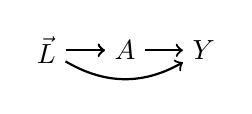
\begin{tikzpicture}
\node (l) at (0,0) {$\vec{L}$};
\node (a) at (1,0) {$A$};
\node (y) at (2,0) {$Y$};
\draw<1-2>[->, thick] (l) -- (a);
\draw<3->[->, thick, dashed] (l) -- (a);
\draw[->, thick] (a) -- (y);
\draw[->, thick] (l) to[bend right] (y);
\end{tikzpicture}
\end{center} \pause
Within each $\vec{L}$, reweight units\\so that every value of $A$ is equally prevalent. \pause
\begin{itemize}
\item Effectively: Remove the dashed edge
\end{itemize} \vskip .2in \pause
In our pseudo-population, the mean given $A = a$ equals the expected outcome under an intervention to set $A= a$
$$\E_{\text{PseudoPopulation}}(Y\mid A = a) = \E(Y^a)$$
\end{frame}

\begin{frame}{Marginal structural models}

Example:
$$\E(Y^a) = \alpha + \beta a$$ \pause
\begin{itemize}
\item Not OLS: Modeling potential rather than factual outcomes \pause
\item Assume a functional form on the thing you will report \pause
\item Deal with confounding by inverse probability weights \pause
\item Gains efficiency by pooling information across treatments \pause
\begin{itemize}
\item Very useful when treatment has sparse values
\end{itemize}
\end{itemize} \pause \vskip .2in
To estimate:
$$\E(Y^a) = \E_\text{PsuedoPopulation}(Y\mid A = a) = \alpha + \beta a$$
This is OLS weighted to the pseudo-population
\end{frame}

\begin{frame}{Marginal structural models: Concrete steps}

\begin{enumerate} \pause
\item Assume a DAG where $\vec{L}$ blocks backdoor paths \pause
\item Estimate inverse probability weights
$$\hat{w}_i = \frac{1}{\hat\P(A = a_i\mid \vec{L} = \vec\ell_i)}$$ \pause
\item Assume a functional form
$$\E(Y^a) = f(a)\quad\text{for some simple function }f()$$ 
\begin{itemize}
\item Example: $\E(Y^a) = \alpha + \beta a$
\item ``marginal'': only modeling as a function of $a$, not $\vec{L}$
\item ``structural'': causal response to an intervention on $A$
\end{itemize} \pause
\item Estimate $\hat\E(Y^a)$: Weighted regression of $Y$ on $A$, using $\hat{w}$
\end{enumerate}

\end{frame}

\begin{frame}{Stabilized weights}
Standard weights can be high-variance: denominator is small
$$w_i = \frac{1}{\P(A = a_i\mid \vec{L} = \vec\ell_i)}$$ \pause \vskip .2in
Stabilized weights can have lower variance
$$w_i = \frac{P(A = a_i)}{\P(A = a_i\mid \vec{L} = \vec\ell_i)}$$ \pause \vskip .2in
This yields efficiency gains only for when the model for $\E(Y^a)$ is not saturated (Hern\'an \& Robins p. 158)
\end{frame}

\begin{frame}{Word of warning: Continuous treatments}

When $A$ is continuous, pooling information over $A$ is appealing.\vskip .1in \pause
A marginal structural model is possible
$$w_i = \frac{1}{f_{A\mid\vec{L}_i}(a_i)}$$
where $f_{A\mid\vec{L}_i}(a_i)$ is the conditional \emph{density} of $A$ given $\vec{L}$. \pause \vskip .2in
But densities are hard to estimate
\begin{itemize}
\item Requires not just the mean---the whole distribution
\item Can be very sensitive
\end{itemize}
\vskip .2in \pause
See Hern\'an \& Robins 12.4.

\end{frame}

\goalsframe

\begin{frame}{Let me know what you are thinking}

\begin{huge} \bref{https://tinyurl.com/CausalQuestions}{tinyurl.com/CausalQuestions} \end{huge}
\vskip .7in

Office hours TTh 11am-12pm and at \bref{https://calendly.com/ianlundberg/office-hours}{calendly.com/ianlundberg/office-hours}\\Come say hi!

\end{frame}

\end{document}